\chapter{The Photon in the Standard Model of Particle Physics}
\index{Photon}\index{Standard Model of Particle Physics}
\setcounter{section}{8}
\setcounter{subsection}{0}
\setcounter{subsubsection}{1}
\setcounter{secnumdepth}{3}
% Box style definitions
\tcbset{physikbox/.style={colback=blue!5!white, colframe=blue!75!black, fonttitle=\bfseries}}
\tcbset{mathebox/.style={colback=green!5!white, colframe=green!50!black, fonttitle=\bfseries}}
\tcbset{didaktikbox/.style={colback=yellow!5!white, colframe=yellow!50!black, fonttitle=\bfseries}}
\tcbset{hypobox/.style={colback=orange!5!white, colframe=orange!75!black, fonttitle=\bfseries}}
\tcbset{hinweisbox/.style={colback=gray!10!white, colframe=black!40!black, fonttitle=\bfseries}}

\subsection{The Standard Model: Overview}
\index{Gravitation}\index{Quantum Electrodynamics (QED)}\index{Weak Interaction}\index{Quantum Chromodynamics (QCD)}\index{Fermion}\index{Boson}\index{Gauge boson}\index{Higgs boson}\index{Higgs mechanism}\index{Gauge symmetry}\index{Lie group}\index{SU(3)}\index{SU(2)}\index{U(1)}\index{Electroweak theory}\index{Dark Matter}\index{Dark Energy}

The \textbf{Standard Model of Particle Physics} is a highly successful theory that describes the known fundamental particles and their interactions—with the exception of \textbf{gravitation}.  
It combines \textbf{quantum electrodynamics (QED)}, the \textbf{quantum theory of the weak interaction}, and \textbf{quantum chromodynamics (QCD)} into a consistent framework.

The fundamental building blocks are \textbf{fermions}, which form matter, and \textbf{bosons}, which act as exchange particles for the fundamental forces.  
Bosons are particles with integer spin that mediate the fundamental interactions.  
The gauge bosons include the \textbf{photon} (carrier of the electromagnetic interaction), the \textbf{$W^\pm$ and $Z^0$ bosons} (carriers of the weak interaction), and the \textbf{gluons} (carriers of the strong interaction).  
The \textbf{Higgs boson} plays a special role: it gives elementary particles their mass through the \textbf{Higgs mechanism}.

The interactions are described by \textbf{gauge symmetries}, formulated in the mathematical language of \textbf{Lie groups}.  
The Standard Model is based on the symmetry group \(\mathrm{SU(3)} \times \mathrm{SU(2)} \times \mathrm{U(1)}\).  
Each factor corresponds to a fundamental interaction:  
\(\mathrm{SU(3)}\) for the strong interaction, \(\mathrm{SU(2)} \times \mathrm{U(1)}\) for the \textbf{electroweak theory}.

Despite its success, the Standard Model is incomplete:  
It explains neither gravitation nor the nature of \textbf{dark matter} or \textbf{dark energy}.

\subsection{U(1) Gauge Symmetry and the Photon}
\index{U(1) gauge symmetry}\index{Abelian group}\index{Global symmetry}\index{Noether theorem}\index{Charge conservation}\index{Local symmetry}\index{Electromagnetic potential}\index{Gauge coupling}\index{Abelian gauge theory}

The electromagnetic interaction can be elegantly formulated as a \textbf{U(1) gauge symmetry}.  
The group \(\mathrm{U(1)}\) consists of all complex numbers of absolute value 1, expressed as \(e^{i\theta}\).  
It is an \textbf{abelian group}, i.e. the group operation (here: multiplication) is commutative.  
In mathematics, \(\mathrm{U(1)}\) is a \textbf{Lie group}, a continuous symmetry group parametrized by continuous parameters.

In quantum mechanics, a \textbf{global U(1) symmetry} describes the invariance of the wave function under a phase change \(\psi \to e^{i\alpha}\psi\).  
According to \textbf{Noether’s theorem}, this symmetry is directly linked to \textbf{charge conservation}.

If the symmetry is made \emph{local}—i.e. the phase angle \(\alpha\) may depend on space and time—one speaks of a \textbf{local U(1) gauge symmetry}.  
To preserve this invariance, a new field must be introduced: the electromagnetic potential \(A_\mu\).  
This field compensates the phase changes and leads to the \textbf{gauge coupling} between charged particles and the field.

Quantizing this field yields the \textbf{photon} as the massless \textbf{gauge boson} of the electromagnetic interaction.  
Its properties—especially masslessness and spin 1—follow directly from the structure of the U(1) symmetry.

The U(1) gauge theory is a special case of an abelian gauge theory and forms the electromagnetic sector of the \textbf{electroweak theory}.  
Its mathematical simplicity makes it an ideal starting point for understanding more complex theories such as \(\mathrm{SU(2)}\) or \(\mathrm{SU(3)}\).

\vspace{1em}
\begin{tcolorbox}[didaktikbox, title=U(1) explained intuitively]
	\label{box:u1_kreis}
	\small
	\begin{minipage}{0.35\textwidth}
		\centering
		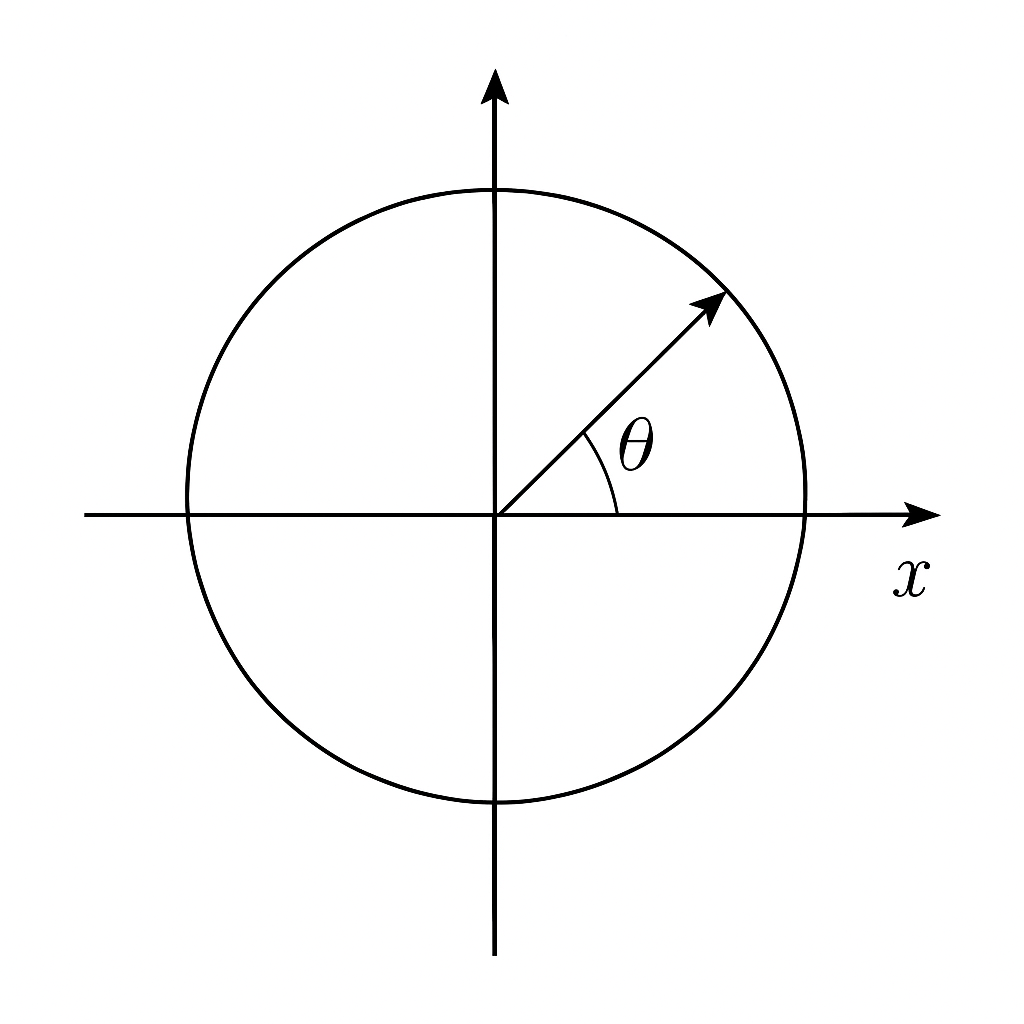
\includegraphics[width=\linewidth]{bilder/u1_kreis.png}
	\end{minipage}%
	\begin{minipage}{0.63\textwidth}
		The group \(\mathrm{U(1)}\) can be pictured as all possible 
		rotations on a circle.  
		Each point on the circle is defined by an angle \(\theta\).  
		In quantum mechanics this corresponds to a phase change of the wave function
		– the distance to the origin always stays the same, only the direction changes.
	\end{minipage}
\end{tcolorbox}

\subsection{Electroweak Unification}
\index{Electroweak theory}\index{Glashow, Sheldon}\index{Salam, Abdus}\index{Weinberg, Steven}\index{Nobel Prize in Physics}\index{SU(2)}\index{Weinberg angle}\index{Higgs mechanism}\index{CERN}

The \textbf{electroweak theory} unifies the \textbf{electromagnetic interaction} and the \textbf{weak interaction} in a single theoretical framework.  
It was developed in the late 1960s by \textbf{Sheldon Glashow}, \textbf{Abdus Salam}, and \textbf{Steven Weinberg} and forms a central part of the \textbf{Standard Model of Particle Physics}.  
For this achievement they received the \textbf{Nobel Prize in Physics} in 1979.

Mathematically, the electroweak theory is based on the symmetry group \(\mathrm{SU(2)} \times \mathrm{U(1)}\).  
The \(\mathrm{SU(2)}\) symmetry describes the weak interaction with its three gauge bosons \(W^1, W^2, W^3\), while the \(\mathrm{U(1)}\) symmetry represents the electromagnetic part.  
Through a mixing (\emph{Weinberg angle}) of the fields \(W^3\) and \(B\) (the U(1) boson), the massless \textbf{photon} and the neutral \textbf{\(Z^0\) boson} emerge.

The electroweak symmetry is spontaneously broken by the \textbf{Higgs mechanism}.  
This gives the \(W^\pm\) and \(Z^0\) bosons mass, while the photon remains massless.  
This property is a direct manifestation of the remaining unbroken U(1) symmetry of electrodynamics.

The experimental confirmation of the electroweak theory came in the early 1980s at \textbf{CERN} through the direct detection of the \(W\) and \(Z\) bosons.  
This discovery is regarded as one of the greatest successes of modern particle physics.

\vspace{1em}
\begin{tcolorbox}[didaktikbox, title=From \(W^3\) and \(B\) to the Photon]
	\label{box:weinberg_mischung}
	\small
	\begin{minipage}{0.35\textwidth}
		\centering
		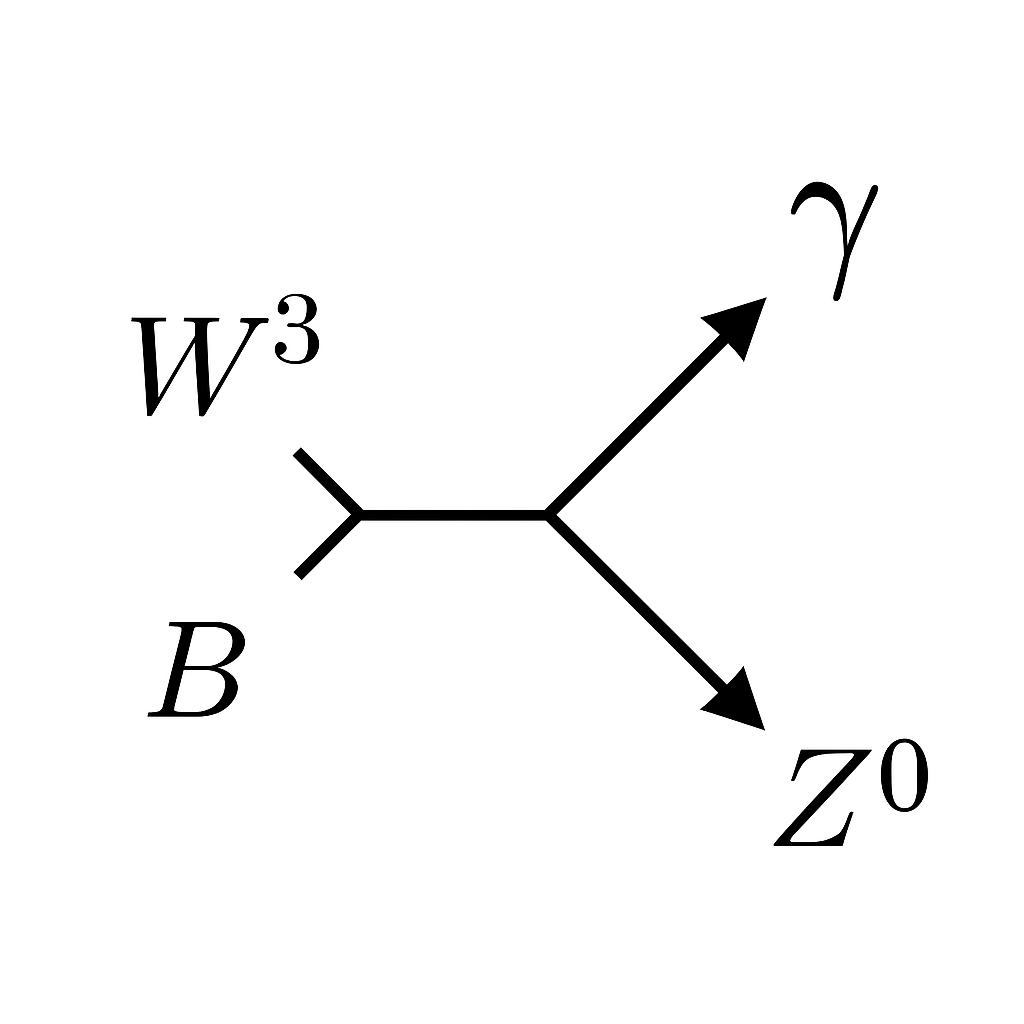
\includegraphics[width=\linewidth]{bilder/weinberg_mischung.png}
	\end{minipage}%
	\begin{minipage}{0.63\textwidth}
		In electroweak theory, the \textbf{photon} \(\gamma\) and the neutral 
		\(\mathbf{Z^0}\) boson arise through a mixing of the fields \(W^3\) and \(B\) 
		– described by the \textbf{Weinberg angle} \(\theta_W\).  
		\vspace{0.3em}
		
		Mathematically:
		\[
		\begin{aligned}
			\gamma &= \phantom{-}\cos\theta_W \, B + \sin\theta_W \, W^3 \\
			Z^0    &= -\sin\theta_W \, B + \cos\theta_W \, W^3
		\end{aligned}
		\]
		This rotation of fields explains why the photon remains massless, while 
		the \(Z^0\) boson acquires mass.
	\end{minipage}
\end{tcolorbox}
\newpage
\noindent
\subsection{Why Is the Photon Massless?}
\index{Photon mass}\index{Lagrangian density}\index{Range of electromagnetic interaction}\index{Compton wavelength}

Within the \textbf{Standard Model of Particle Physics}, the \textbf{photon} is a massless \textbf{gauge boson} of the electromagnetic interaction.  
Its masslessness is a direct consequence of the unbroken \textbf{U(1) gauge symmetry} in \textbf{quantum electrodynamics (QED)}.

In the \textbf{Higgs mechanism}, which gives the \(W^\pm\) and \(Z^0\) bosons mass, exactly one gauge symmetry remains unbroken: the U(1) symmetry of electrodynamics.  
The associated gauge field is identified with the photon—and since unbroken gauge symmetries always lead to massless exchange particles, the photon has no rest mass.

Mathematically this appears in the Lagrangian density of the electromagnetic field: no mass term of the form \(\frac{1}{2} m^2 A_\mu A^\mu\) occurs.  
Such a term would violate gauge invariance and is therefore forbidden.

Experimental bounds on a possible photon mass are extremely strict:  
Measurements set an upper limit of less than \(10^{-18}\,\mathrm{eV}/c^2\).  
Practically the photon is perfectly massless—an essential property for the infinite range of the electromagnetic force.

\vspace{1em}
\begin{tcolorbox}[hinweisbox, title=Masslessness and range]
	\label{box:reichweite_masselos}
	\small
	The range of a fundamental interaction is directly linked to the mass of its exchange particle.  
	\begin{itemize}
		\item \textbf{Massless exchange particles} (e.g. photons) mediate forces with unlimited range.  
		\item \textbf{Massive exchange particles} (e.g. \(W^\pm\) and \(Z^0\) bosons) mediate forces with finite range, determined by the \emph{Compton wavelength} \(\lambda_C = \hbar/(mc)\).
	\end{itemize}
	For the photon, its masslessness implies the infinite range of the electromagnetic interaction.
\end{tcolorbox}
\newpage
\noindent
\vspace{1em}
\begin{tcolorbox}[physikbox, title=Massless photon and spin correlations over long distances]
	\label{box:photon_spin_reichweite}
	\small
	A massless photon has no range limitation in transmitting its quantized properties.  
	This has two essential consequences:
	\begin{itemize}
		\item \textbf{Infinite interaction range:} The electromagnetic force acts in principle over arbitrary distances.
		\item \textbf{Conservation of spin direction (polarization):} Since the photon is massless and travels at the speed of light, its spin or polarization orientation is preserved even across cosmological distances. 
	\end{itemize}
	In entangled quantum states this means that the polarization correlations of two photons remain measurable even when they are far apart—a result of the combination of masslessness and quantum entanglement.
\end{tcolorbox}

\subsection{Comparison with Other Gauge Bosons}
\index{W boson}\index{Z boson}\index{Gluon}\index{Confinement}\index{Graviton}

In the \textbf{Standard Model of Particle Physics} there are several \textbf{gauge bosons} that mediate fundamental interactions.  
The \textbf{photon} differs from them in essential properties:

\begin{itemize}
	\item \textbf{Photon (QED):} Massless, spin \(1\), mediates the \textbf{electromagnetic interaction}.  
	Range: infinite.
	
	\item \(\mathbf{W^\pm}\) and \(\mathbf{Z^0}\) \textbf{bosons} (electroweak theory):  
	Spin \(1\), heavy masses (\(\approx 80{-}91\,\mathrm{GeV}/c^2\)), range: about \(10^{-18}\,\mathrm{m}\).  
	Mediators of the \textbf{weak interaction}.
	
	\item \textbf{Gluons} (QCD):  
	Spin \(1\), formally massless, mediate the \textbf{strong interaction}.  
	Effective range is very limited due to \textbf{confinement}—gluons never appear as free particles.
	
	\item \textbf{Graviton} (hypothetical):  
	Spin \(2\), massless, would mediate gravitation.  
	Not experimentally confirmed.
\end{itemize}

The decisive difference:  
Only the photon appears as a freely measurable, massless exchange particle with unlimited range.  
W and Z bosons are massive and thus short-range, gluons are massless but confined in bound states.

\vspace{1em}
\begin{tcolorbox}[hinweisbox, title=Comparison of gauge bosons]
	\label{box:eichbosonen_vergleich}
	\small
	
	\resizebox{\linewidth}{!}{%
		\begin{tabular}{lcccc}
			\textbf{Particle} & \textbf{Spin} & \textbf{Mass} & \textbf{Range} & \textbf{Interaction} \\
			\hline
			Photon & 1 & 0 & infinite & electromagnetic \\
			\(W^\pm\) & 1 & \(\approx 80\,\mathrm{GeV}/c^2\) & \(10^{-18}\,\mathrm{m}\) & weak \\
			\(Z^0\) & 1 & \(\approx 91\,\mathrm{GeV}/c^2\) & \(10^{-18}\,\mathrm{m}\) & weak \\
			Gluon & 1 & 0 & \emph{effectively short} & strong (confinement) \\
			Graviton (hyp.) & 2 & 0 & infinite & gravitation \\
		\end{tabular}%
	}
	
\end{tcolorbox}

\subsection{Open Questions and Extensions}
\index{Grand Unified Theory (GUT)}\index{String theory}\index{Quantum gravity}

Despite the success of the \textbf{Standard Model of Particle Physics}, fundamental questions remain unanswered that also involve the \textbf{photon} or could extend its theoretical framework:

\begin{itemize}
	\item \textbf{Photon mass:}  
	Experimentally the photon is considered massless, but an extremely tiny, so far unmeasurable mass cannot be excluded.  
	Future precision measurements may further constrain this limit—or surprisingly reveal a finite mass.
	
	\item \textbf{Interaction with dark matter:}  
	Whether photons couple in any way to dark matter is unknown.  
	Direct and indirect searches may provide hints in the future.
	
	\item \textbf{Unified theories:}  
	In models beyond the Standard Model—such as \textbf{Grand Unified Theories (GUT)} or \textbf{string theories}—the photon is part of a larger symmetry structure.  
	These models may predict new properties or partner particles.
	
	\item \textbf{Quantum gravity:}  
	A consistent theory uniting gravitation with the quantum fields of particle physics is still missing.  
	The interaction of the photon with hypothetical \textbf{gravitons} or with the structure of spacetime on the smallest scales remains largely unexplored.
	
	\item \textbf{New symmetries or particles:}  
	Extensions of the Standard Model could involve additional gauge bosons or symmetries that influence the role of the photon.
\end{itemize}

Answering these questions will require a combination of precise experiments, new observational technologies, and theoretical breakthroughs.  
Thus, the photon remains not only a central tool of physics but also a key to possible new physical worlds.

\subsection{Conclusion}
\subsubsection*{The Photon – Particle, Wave, and Window to the Future}
\phantomsection
The \textbf{photon} has played a unique role in the history of physics:  
It was the key to the birth of quantum theory, the starting point for the development of \textbf{quantum electrodynamics (QED)}, and remains an indispensable tool of both experimental and theoretical research.

From the \textbf{photoelectric effect} to \textbf{Compton scattering} to modern applications such as \textbf{quantum communication} and \textbf{photonics}, the photon has not only shaped our physical models but also enabled technologies that transform daily life.

Within the \textbf{Standard Model of Particle Physics}, the photon embodies an unbroken \textbf{U(1) gauge symmetry}—a mathematical elegance expressed in its masslessness and infinite range.  
At the same time, the open questions show that we are still far from a complete understanding.


The photon unites fundamental properties of nature:
\begin{itemize}
	\item \textbf{Wave and particle} in a single quantum description.
	\item \textbf{Massless messenger} with infinite range.
	\item \textbf{Precise probe} in astronomy, particle physics, and quantum optics.
	\item \textbf{Key actor} in future technologies such as quantum computers and photonic circuits.
\end{itemize}

Its dual role as theoretical foundation and practical tool makes the photon one of the most fascinating objects in physics.  
It is not only a component of our physical worldview but also a gateway to yet unknown aspects of the universe—a gateway that we will continue to push open in the decades ahead.

Even though the photon appears in a clear and consistent role in the Standard Model, 
it simultaneously symbolizes the limits of this theory.  
To highlight this dual function—as foundation and as bridge to new physics— 
we conclude with a didactic summary and then take a speculative look into the future.
\newpage
\noindent
\vspace{1em}
\begin{tcolorbox}[didaktikbox, title=Didactic conclusion: The photon in the Standard Model]
	\label{box:didaktik_kapVIII}
	The photon is not only a tool of quantum optics and modern technology, 
	but also a key figure in the theoretical foundation of physics.  
	
	\medskip
	\textbf{Core message:}  
	Its role as a massless gauge boson of the unbroken U(1) symmetry combines mathematical elegance, 
	experimental precision, and cosmic range.  
	Thus the photon exemplifies both the strength—and the limits—of the Standard Model.
\end{tcolorbox}

\vspace{1em}
\begin{tcolorbox}[hypobox, title={What if the Standard Model were only a stepping stone?}]
	\label{Merksatz zum Photon}
	A thought experiment:
	\begin{itemize}
		\item If photons could interact with dark matter, our understanding of cosmology would be revolutionized.  
		\item Detecting a tiny photon mass would fundamentally change the structure of electrodynamics.  
		\item New symmetries or hidden partner particles of the photon could appear in an extended theory beyond the Standard Model.  
		\item Perhaps the photon is even the key to linking quantum field theory and gravitation.  
	\end{itemize}
	
	\medskip
	Such speculative perspectives go beyond the Standard Model—and open the door 
	to a future chapter on \emph{new physics}.
\end{tcolorbox}
